\documentclass[a4paper, 12pt]{article}

% packages
\usepackage{amssymb}
\usepackage[fleqn]{mathtools}
\usepackage{tikz}
\usepackage{enumerate}
\usepackage{bussproofs}
\usepackage{xcolor}
\usepackage[margin=1.3cm]{geometry}
\usepackage{logicproof}
\usepackage{diagbox}
\usepackage{listings}
\usepackage{graphicx}
\usepackage{lstautogobble}
\usepackage{hyperref}
\usepackage{multirow}
\usepackage{tipa}
\usepackage{pgfplots}

% tikz libraries
\usetikzlibrary{
    decorations.pathreplacing,
    arrows,
    shapes.gates.logic.US,
    circuits.logic.US,
    calc,
    automata,
    positioning,
    intersections
}

\pgfplotsset{compat=1.16}

\pgfmathdeclarefunction{gauss}{2}{%
  \pgfmathparse{1/(#2*sqrt(2*pi))*exp(-((x-#1)^2)/(2*#2^2))}%
}

\allowdisplaybreaks % allow environments to break
\setlength\parindent{0pt} % no indent

% shorthand for verbatim
% this clashes with logicproof, so maybe fix this at some point?
\catcode`~=\active
\def~#1~{\texttt{#1}}

% code listing
\lstdefinestyle{main}{
    numberstyle=\tiny,
    breaklines=true,
    showspaces=false,
    showstringspaces=false,
    tabsize=2,
    numbers=left,
    basicstyle=\ttfamily,
    columns=fixed,
    fontadjust=true,
    basewidth=0.5em,
    autogobble,
    xleftmargin=3.0ex,
    mathescape=true
}
\newcommand{\dollar}{\mbox{\textdollar}} %
\lstset{style=main}

% augmented matrix
\makeatletter
\renewcommand*\env@matrix[1][*\c@MaxMatrixCols c]{%
\hskip -\arraycolsep
\let\@ifnextchar\new@ifnextchar
\array{#1}}
\makeatother

% ceiling / floor
\DeclarePairedDelimiter{\ceil}{\lceil}{\rceil}
\DeclarePairedDelimiter{\floor}{\lfloor}{\rfloor}

% custom commands
\newcommand{\indefint}[2]{\int #1 \, \mathrm{d}#2}
\newcommand{\defint}[4]{\int_{#1}^{#2} #3 \, \mathrm{d}#4}
\newcommand{\pdif}[2]{\frac{\partial #1}{\partial #2}}
\newcommand{\dif}[2]{\frac{\mathrm{d}#1}{\mathrm{d}#2}}
\newcommand{\limit}[2]{\raisebox{0.5ex}{\scalebox{0.8}{$\displaystyle{\lim_{#1 \to #2}}$}}}
\newcommand{\limitsup}[2]{\raisebox{0.5ex}{\scalebox{0.8}{$\displaystyle{\limsup_{#1 \to #2}}$}}}
\newcommand{\summation}[2]{\sum\limits_{#1}^{#2}}
\newcommand{\product}[2]{\prod\limits_{#1}^{#2}}
\newcommand{\intbracket}[3]{\left[#3\right]_{#1}^{#2}}
\newcommand{\laplace}{\mathcal{L}}
\newcommand{\fourier}{\mathcal{F}}
\newcommand{\mat}[1]{\boldsymbol{#1}}
\renewcommand{\vec}[1]{\boldsymbol{#1}}
\newcommand{\rowt}[1]{\begin{bmatrix}
    #1
\end{bmatrix}^\top}
\DeclareMathOperator*{\argmax}{argmax}
\DeclareMathOperator*{\argmin}{argmin}

\newcommand{\lto}[0]{\leadsto\ }

\newcommand{\ulsmash}[1]{\underline{\smash{#1}}}

\newcommand{\powerset}[0]{\wp}
\renewcommand{\emptyset}[0]{\varnothing}

\makeatletter
\newsavebox{\@brx}
\newcommand{\llangle}[1][]{\savebox{\@brx}{\(\m@th{#1\langle}\)}%
  \mathopen{\copy\@brx\kern-0.5\wd\@brx\usebox{\@brx}}}
\newcommand{\rrangle}[1][]{\savebox{\@brx}{\(\m@th{#1\rangle}\)}%
  \mathclose{\copy\@brx\kern-0.5\wd\@brx\usebox{\@brx}}}
\makeatother
\newcommand{\lla}{\llangle}
\newcommand{\rra}{\rrangle}
\newcommand{\la}{\langle}
\newcommand{\ra}{\rangle}
\newcommand{\crnr}[1]{\text{\textopencorner} #1 \text{\textcorner}}
\newcommand{\bnfsep}[0]{\ |\ }
\newcommand{\concsep}[0]{\ ||\ }

\newcommand{\axiom}[1]{\AxiomC{#1}}
\newcommand{\unary}[1]{\UnaryInfC{#1}}
\newcommand{\binary}[1]{\BinaryInfC{#1}}
\newcommand{\trinary}[1]{\TrinaryInfC{#1}}
\newcommand{\quaternary}[1]{\QuaternaryInfC{#1}}
\newcommand{\quinary}[1]{\QuinaryInfC{#1}}
\newcommand{\dproof}[0]{\DisplayProof}

\newcommand{\ttbs}{\char`\\}
\newcommand{\lrbt}[0]{\ \bullet\ }

% colours
\newcommand{\violet}[1]{\textcolor{violet}{#1}}
\newcommand{\blue}[1]{\textcolor{blue}{#1}}
\newcommand{\red}[1]{\textcolor{red}{#1}}
\newcommand{\teal}[1]{\textcolor{teal}{#1}}

% reasoning proofs
\usepackage{ltablex}
\usepackage{environ}
\keepXColumns
\NewEnviron{reasoning}{
    \begin{tabularx}{\textwidth}{rlX}
        \BODY
    \end{tabularx}
}
\newcommand{\proofline}[3]{$(#1)$ & $#2$ & \hfill #3 \smallskip \\}
\newcommand{\proofarbitrary}[1]{& take arbitrary $#1$ \smallskip \\}
\newcommand{\prooftext}[1]{\multicolumn{3}{l}{#1} \smallskip \\}
\newcommand{\proofmath}[3]{$#1$ & = $#2$ & \hfill #3 \smallskip \\}
\newcommand{\prooftherefore}[1]{& $\therefore #1$ \smallskip \\}
\newcommand{\proofbc}[0]{\prooftext{\textbf{Base Case}}}
\newcommand{\proofis}[0]{\prooftext{\textbf{Inductive Step}}}

% ER diagrams
\newcommand{\nattribute}[4]{
    \node[draw, state, inner sep=0cm, minimum size=0.2cm, label=#3:{#4}] (#1) at (#2) {};
}
\newcommand{\mattribute}[4]{
    \node[draw, state, accepting, inner sep=0cm, minimum size=0.2cm, label=#3:{#4}] (#1) at (#2) {};
}
\newcommand{\dattribute}[4]{
    \node[draw, state, dashed, inner sep=0cm, minimum size=0.2cm, label=#3:{#4}] (#1) at (#2) {};
}
\newcommand{\entity}[3]{
    \node[] (#1-c) at (#2) {#3};
    \node[inner sep=0cm] (#1-l) at ($(#1-c) + (-1, 0)$) {};
    \node[inner sep=0cm] (#1-r) at ($(#1-c) + (1, 0)$) {};
    \node[inner sep=0cm] (#1-u) at ($(#1-c) + (0, 0.5)$) {};
    \node[inner sep=0cm] (#1-d) at ($(#1-c) + (0, -0.5)$) {};
    \draw
    ($(#1-c) + (-1, 0.5)$) -- ($(#1-c) + (1, 0.5)$) -- ($(#1-c) + (1, -0.5)$) -- ($(#1-c) + (-1, -0.5)$) -- cycle;
}
\newcommand{\relationship}[3]{
    \node[] (#1-c) at (#2) {#3};
    \node[inner sep=0cm] (#1-l) at ($(#1-c) + (-1, 0)$) {};
    \node[inner sep=0cm] (#1-r) at ($(#1-c) + (1, 0)$) {};
    \node[inner sep=0cm] (#1-u) at ($(#1-c) + (0, 1)$) {};
    \node[inner sep=0cm] (#1-d) at ($(#1-c) + (0, -1)$) {};
    \draw
    ($(#1-c) + (-1, 0)$) -- ($(#1-c) + (0, 1)$) -- ($(#1-c) + (1, 0)$) -- ($(#1-c) + (0, -1)$) -- cycle;
}

% AVL Trees
\newcommand{\avltri}[4]{
    \draw ($(#1)$) -- ($(#1) + #4*(0.5, -1)$) -- ($(#1) + #4*(-0.5, -1)$) -- cycle;
    \node at ($(#1) + #4*(0, -1) + (0, 0.5)$) {#3};
    \node at ($(#1) + #4*(0, -1) + (0, -0.5)$) {#2};
}

% RB Trees
\tikzset{rbtr/.style={inner sep=2pt, circle, draw=black, fill=red}}
\tikzset{rbtb/.style={inner sep=2pt, circle, draw=black, fill=black}}

% actual document
\begin{document}
    \section*{CO220 - Software Engineering Design}
        \subsection*{8th October 2019}
            \subsubsection*{Cost of Change}
                \begin{center}
                    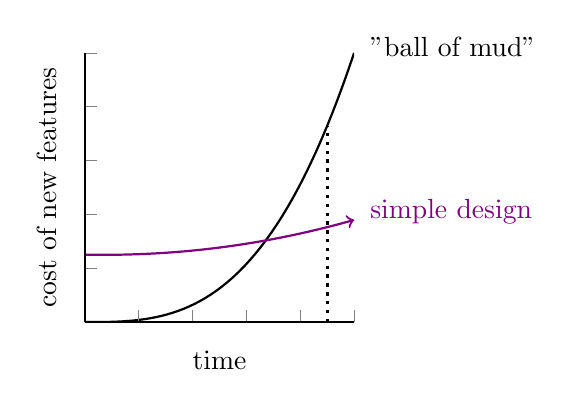
\begin{tikzpicture}
                        \begin{axis}[
                            axis on top=true,
                            axis line style=thick,
                            no markers, domain=0:10, samples=50,
                            axis lines*=left, xlabel={time}, ylabel={cost of new features},
                            height=5cm, width=5cm,
                            enlargelimits=false,
                            xticklabels={,,},
                            yticklabels={,,}
                        ]
                            \addplot[mark=none, black, very thick, dotted] coordinates {(9, 0) (9, 729)};
                            \addplot[thick] {\x^3};
                            \addplot[violet, thick, ->] {250+\x^1.75*ln(\x)};
                        \end{axis}
                        \node[anchor=west] at (3.5, 3.5) {"ball of mud"};
                        \node[anchor=west] at (3.5, 1.4) {\violet{simple design}};
                    \end{tikzpicture}
                \end{center}
                The "project heat death", denoted by the dotted line, is where the cost of adding new features outweighs the value gained by adding those features.
                Note that the initial cost of doing a simple design can be more expensive (since it requires more planning).
            \subsubsection*{Elements of Simple Design}
                This is arranged in a pyramid on the slides (since they "build up on each other") but I will write it as a list, starting from the bottom;
                \begin{enumerate}[1.]
                    \itemsep0em
                    \item \textbf{behaves correctly}
                        \medskip

                        It doesn't matter if the codebase is well structured, or the code is elegant if it doesn't do the right thing (is buggy, or isn't what the customer wanted).
                        \begin{itemize}
                            \itemsep0em
                            \item automated testing
                            \item test-driven development
                            \item mock objects
                        \end{itemize}
                    \item \textbf{minimises duplication}
                        \medskip

                        If something needs to be changed in the future, and it's in multiple places, it will have to be changed in all of those places which will take longer.
                        Additionally, it's also easy to miss, causing bugs.
                    \item \textbf{maximises clarity}
                        \medskip

                        Code should be easy to modify, such that the parts that need to be changed can be easily located.
                        Important especially if working with others.
                    \item \textbf{has fewer elements}
                        \medskip

                        Less important - we want to focus on the previous levels first, and don't want to lose the benefits by combining elements.
                \end{enumerate}
            \subsubsection*{Test-Driven Development / Behaviour Driven Development}
                Having a test suite provides confidence that the codebase still works, even after major changes.
                \begin{center}
                    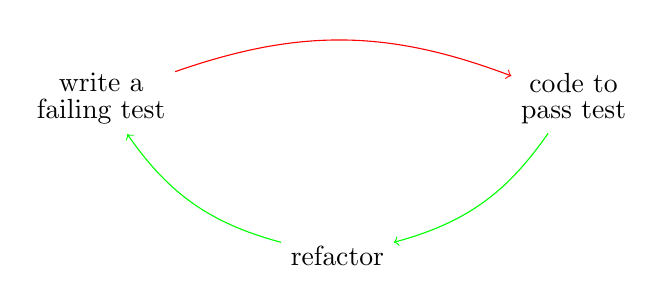
\begin{tikzpicture}[x=3cm]
                        \node (w) at (0, 0) {\shortstack{write a\\failing  test}};
                        \node (c) at (2, 0) {\shortstack{code to\\pass test}};
                        \node (r) at (1, -2) {refactor};
                        \draw
                        (w) edge[red, ->, bend left=20] (c)
                        (c) edge[green, ->, bend left=20] (r)
                        (r) edge[green, ->, bend left=20] (w);
                    \end{tikzpicture}
                \end{center}
                We start by writing failing tests, which seems counterintuitive, as there is no code to test.
                However, these tests are written as if the code was working - which gives us a specification on how the code \textbf{should} behave.
                We want to write code as quickly as possible that gets us from the \red{red} state (failing tests), to a \textcolor{green}{green} state (passing tests).
                This code is likely untidy - we can then tidy it up (which shouldn't break the tests).
                \medskip

                Additionally, it's not only about testing; we can replace the stages as follows;
                \begin{itemize}
                    \itemsep0em
                    \item API design \hfill (write a failing test)
                        \subitem "I wish there was a method that would take these parameters and do this"
                    \item internals design \hfill (code to pass test)
                        \subitem "Just making it work"
                    \item structural design \hfill (refactor)
                        \subitem "How can we improve the design?" (pyramid layers)
                \end{itemize}
                We focus more on what it should do (how it should behave), and not how it does it.
                For example, ~CustomerLookup~ should do the following;
                \begin{itemize}
                    \itemsep0em
                    \item finds customer by ID
                    \item fails for duplicate customers
                \end{itemize}
                The test is named as the expected result, and if it is true, then it behaves correctly.
                \begin{lstlisting}
                    public class CustomerLookupTest {
                      @Test
                      findsCustomerById() {
                        ...
                      }
                      @Test
                      failsForDuplicateCustomers() {
                        ...
                      }
                    }
                \end{lstlisting}
            \subsubsection*{Example of TDD}
                The object ~FibonacciSequence~ should do the following;
                \begin{itemize}
                    \itemsep0em
                    \item defines the first two terms to be one
                    \item has each term equal to the sum of the previous two
                    \item is not defined for negative terms
                \end{itemize}
                \begin{lstlisting}
                    ... // (FibonacciSequenceTest.java)

                    import static org.hamcrst.CoreMatchers.is;
                    import static org,junit.Assert.assertThat;

                    import org.junit.Test;

                    public class FibonacciSequenceTest {

                      @Test
                      public void definesFirstTwoTermsToBeOne() {
                        assertThat(new FibonacciSeqeunce().term(0), is(1));
                        assertThat(new FibonacciSeqeunce().term(1), is(1));
                      }
                    }
                \end{lstlisting}
                Obviously, none of this will work yet, as the code doesn't exist.
                However, we can use this to create the code as follows (this is incorrect, but our tests now pass);
                \begin{lstlisting}
                    ... // (FibonacciSequence.java)

                    public class FibonacciSequence {

                      public int term(int i) {
                        return 1;
                      }
                    }
                \end{lstlisting}
                We can then add more tests, which should now fail;
                \begin{lstlisting}
                    ... // (FibonacciSequenceTest.java)

                    public class FibonacciSequenceTest {
                      ...

                      @Test
                      public void hasEachTermTheSumOfPreviousTwo() {
                        assert(new FibonacciSeqeunce().term(2), is(2));
                        assert(new FibonacciSeqeunce().term(3), is(3));
                        assert(new FibonacciSeqeunce().term(4), is(5));
                      }
                    }
                \end{lstlisting}
                Similarly, we can modify the code again to add a naive implementation which performs it recursively;
                \begin{lstlisting}
                    ... // (FibonacciSequence.java)

                    public class FibonacciSequence {

                      public int term(int i) {
                        if (i < 2) {
                          return 1;
                        }
                        return term(i - 1) + term(i - 2);
                      }
                    }
                \end{lstlisting}
                Adding the last bullet point as a test;
                \begin{lstlisting}
                    ... // (FibonacciSequenceTest.java)

                    public class FibonacciSequenceTest {
                      ...

                      @Test
                      public void isNotDefinedForNegativeIndices() {
                        try {
                          new FibonacciSeqeunce().term(-1);
                          fail("should have thrown exception")
                        } catch (IllegalArgumentException iae) {
                          assertThat(iae.getMessage(), containsString("negative index"))
                        }
                      }
                    }
                \end{lstlisting}
                Fixing this, we add the following;
                \begin{lstlisting}
                    ... // (FibonacciSequence.java)

                    public class FibonacciSequence {

                      public int term(int i) {
                        if (i < 0) {
                          throw new IllegalArgumentException("negative index not supported");
                        }

                        ...
                      }
                    }
                \end{lstlisting}
                This is the only time I will actually write out every step, since that's the focus of TDD.
        \subsection*{11th October 2019}
            \subsubsection*{Feedback}
                Note that the names of the test files should be ~SomeObjectTest~, for ~SomeObject~.
                This convention allows the IDE to link the files, as well as having them in alphabetical order.
                Also always use a \textit{jUnit} library function;
                \begin{center}
                    ~assertThat(rul.size(), is(0))~ or ~assertEquals(0, rul.size())~

                    instead of

                    ~assert rul.size() == 0~
                \end{center}
                Generally make the LHS of fields the interface ~List~ instead of ~ArrayList~, and attempt to make it ~private~ and ~final~ (if possible).
                Additionally, any fields are reinitialised automatically by \textit{jUnit}, hence it doesn't need to be reset at the end of each test.
            \subsubsection*{Refactoring}
                This starts with multiple examples on handouts.
                As we're writing new code, we should look out for small changes that can improve the structure of our code.
                \medskip

                We can accumulate "technical debt" by writing code quickly to get a feature working, but we must fix it soon, otherwise it builds up leading to unhygienic code.
                \medskip

                Note that refactoring should be done with tools when possible (such as renaming identifiers), since the tool will be able to analyse the entire codebase to detect where changes need to be made.
                Behaviour should not be changed.
                \medskip

                The example after this is mostly using \textit{IntelliJ} tools wherever possible.
                One note to make is that sometimes it is helpful to get code into a state where it becomes similar enough to other parts of the code, to allow for the tool to do the work.
        \subsection*{15th October 2019}
            \subsubsection*{Sending Messages}
                Instead of considering how objects call methods, it may be beneficial to design how modules communicate with each other ("send messages").
                \medskip

                The idea is that when one object "sends a message", we don't really care how it does it, just that it performs the expected action.
            \subsubsection*{OOP}
                Typically, larger systems are built up of smaller units that work together.
                Some of these will be from the standard library, some of those will be written by us, and some others may be written by third parties.
                \begin{center}
                    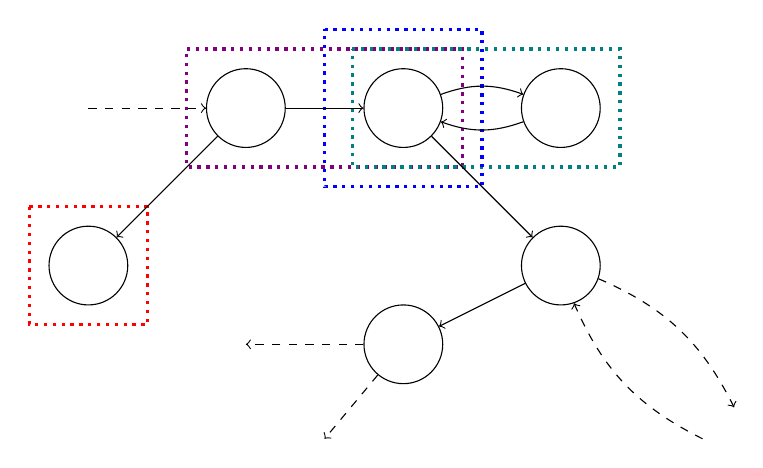
\begin{tikzpicture}[x=2cm, y=2cm]
                        \draw[violet, dotted, very thick] (-0.375, 0.375) -- (1.375, 0.375) -- (1.375, -0.375) -- (-0.375, -0.375) -- cycle;
                        \draw[teal, dotted, very thick] (0.675, 0.375) -- (2.375, 0.375) -- (2.375, -0.375) -- (0.675, -0.375) -- cycle;
                        \draw[red, dotted, very thick] (-1.375, -0.625) -- (-0.625, -0.625) -- (-0.625, -1.375) -- (-1.375, -1.375) -- cycle;
                        \draw[blue, dotted, very thick] (0.5, 0.5) -- (1.5, 0.5) -- (1.5, -0.5) -- (0.5, -0.5) -- cycle;
                        \node[state, minimum size=1cm] (a) at (0, 0) {};
                        \node[state, minimum size=1cm] (b) at (1, 0) {};
                        \node[state, minimum size=1cm] (c) at (2, 0) {};
                        \node[state, minimum size=1cm] (d) at (-1, -1) {};
                        \node[state, minimum size=1cm] (e) at (1, -1.5) {};
                        \node[state, minimum size=1cm] (f) at (2, -1) {};
                        \draw
                        (-1, 0) edge[->, dashed] (a)
                        (a) edge[->] (b)
                        (a) edge[->] (d)
                        (b) edge[->, bend left=20] (c)
                        (b) edge[->] (f)
                        (c) edge[->, bend left=20] (b)
                        (e) edge[->, dashed] (0, -1.5)
                        (e) edge[->, dashed] (0.5, -2.1)
                        (f) edge[->] (e)
                        (f) edge[->, dashed, bend left=20] (3.1, -1.9)
                        (2.9, -2.1) edge[->, dashed, bend left=20] (f);
                    \end{tikzpicture}
                \end{center}
                However, these components should be reusable, and they can be combined in a different way if needed (we can't really modify code in the standard library, etc).
                We want to have the possibility to swap out parts of the project without affecting other objects.
                The system shouldn't care how the object does a job, just that it does it.
                \begin{itemize}
                    \itemsep0em
                    \item \violet{\textbf{commands}} \hfill "please do $X$"
                        \medskip

                        This doesn't wait for a response, or a even a return value.
                    \item \teal{\textbf{queries}} \hfill "please tell me $Y$"
                        \medskip

                        Requests a bit of data, and then processes it.
                        If too many queries are used, we tend to have a central part of the process that deals with all the information which isn't flexible.
                        Ideally jobs are delegated to different components.
                    \item \red{\textbf{value objects}}
                        \medskip

                        These don't typically interact with other objects, and just holds some data and performs some computations.
                        These components can easily be tested.
                    \item \blue{\textbf{tell don't ask}}
                        \medskip

                        The role of this object is to coordinate other objects in the system.
                        Focusing on commands tends to give us more flexibility, but leads to different testing approaches.
                \end{itemize}
                Typically, asking looks like the following (can be characterised by a higher number of ~getX()~s);
                \begin{lstlisting}
                    table.getGrid().getColumnModel().getColumn(index).setPreferredWidth(newWidth);
                \end{lstlisting}
                Visually, the graph becomes something similar to this;
                \begin{center}
                    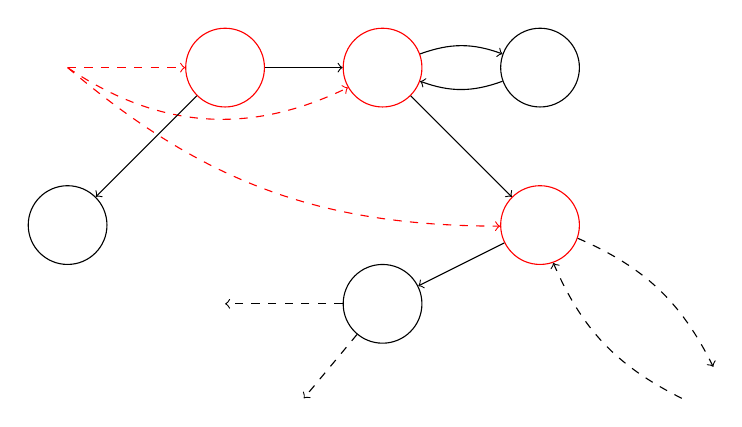
\begin{tikzpicture}[x=2cm, y=2cm]
                        \node[red, state, minimum size=1cm] (a) at (0, 0) {};
                        \node[red, state, minimum size=1cm] (b) at (1, 0) {};
                        \node[state, minimum size=1cm] (c) at (2, 0) {};
                        \node[state, minimum size=1cm] (d) at (-1, -1) {};
                        \node[state, minimum size=1cm] (e) at (1, -1.5) {};
                        \node[red, state, minimum size=1cm] (f) at (2, -1) {};
                        \draw
                        (-1, 0) edge[red, ->, dashed] (a)
                        (-1, 0) edge[red, ->, dashed, bend right=30] (b)
                        (-1, 0) edge[red, ->, dashed, bend right=20] (f)
                        (a) edge[->] (b)
                        (a) edge[->] (d)
                        (b) edge[->, bend left=20] (c)
                        (b) edge[->] (f)
                        (c) edge[->, bend left=20] (b)
                        (e) edge[->, dashed] (0, -1.5)
                        (e) edge[->, dashed] (0.5, -2.1)
                        (f) edge[->] (e)
                        (f) edge[->, dashed, bend left=20] (3.1, -1.9)
                        (2.9, -2.1) edge[->, dashed, bend left=20] (f);
                    \end{tikzpicture}
                \end{center}
            \subsubsection*{Testing Objects and Roles}
                When we want to test a given object, let it be $O$, we shouldn't have to implement the objects it depends on first.
                To do this, we use interfaces in Java to represent roles - which specifies what $O$ expects the other objects to do.
                An object may play different roles (hence implement multiple interfaces).
                \begin{center}
                    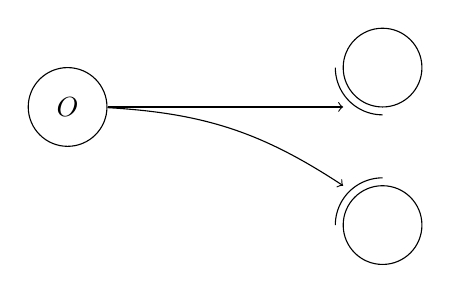
\begin{tikzpicture}
                        \node[state, minimum size=1cm] (a) at (0, 0.5) {$O$};
                        \node[state, minimum size=1cm] at (4, 1) {};
                        \node[state, minimum size=1cm] at (4, -1) {};
                        \draw[black, domain=180:270] plot ({4 + 0.6*cos(\x)}, {1 + 0.6*sin(\x)});
                        \draw[black, domain=90:180] plot ({4 + 0.6*cos(\x)}, {-1 + 0.6*sin(\x)});
                        \draw (a) edge[->, bend left=15] (3.5, -0.5);
                        \draw (a) edge[->] (3.5, 0.5);
                    \end{tikzpicture}
                \end{center}
                The object $O$ is the one we wish to test, and should be triggered by a call in the test suite.
            \subsubsection*{Mock Objects}
                To test objects that rely on stuff other objects that haven't been implemented yet (only an interface exists), we can use mock objects.
                \begin{center}
                    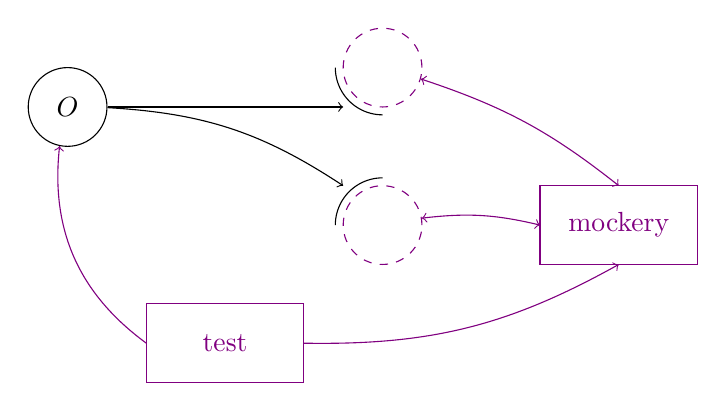
\begin{tikzpicture}
                        \node[state, minimum size=1cm] (a) at (0, 0.5) {$O$};
                        \node[violet, dashed, state, minimum size=1cm] (b) at (4, 1) {};
                        \node[violet, dashed, state, minimum size=1cm] (c) at (4, -1) {};
                        \draw[black, domain=180:270] plot ({4 + 0.6*cos(\x)}, {1 + 0.6*sin(\x)});
                        \draw[black, domain=90:180] plot ({4 + 0.6*cos(\x)}, {-1 + 0.6*sin(\x)});
                        \draw (a) edge[->, bend left=15] (3.5, -0.5);
                        \draw (a) edge[->] (3.5, 0.5);

                        \node[violet] at (2, -2.5) {test};
                        \draw[violet] (1, -2) -- (3, -2) -- (3, -3) -- (1, -3) -- cycle;
                        \draw[violet]
                        (1, -2.5) edge[->, bend left=30] (a)
                        (3, -2.5) edge[->, bend right=15] (7, -1.5)
                        (6, -1) edge[<->, bend right=10] (c)
                        (7, -0.5) edge[<->, bend right=10] (b);
                        \node[violet] at (7, -1) {mockery};
                        \draw[violet] (6, -0.5) -- (8, -0.5) -- (8, -1.5) -- (6, -1.5) -- cycle;
                    \end{tikzpicture}
                \end{center}
                When a test is run, we can test if $O$ sends messages to the mock objects.
                Instead of writing assertions about the state of $O$, we can write expectations for what should be called.
                \medskip

                An example is as follows (this is syntax from \textit{WebSequenceDiagrams}, because I don't want to draw it out);
                \begin{lstlisting}
                    Waiter->HeadChef: order(CHICKEN, APPLE)
                    HeadChef->PastryChef: order(APPLE)

                    Waiter->HeadChef: customerReadyFor(APPLE)
                    HeadChef->PastryChef: isCooked(APPLE)
                    PastryChef-->HeadChef: True
                    HeadChef->Waiter: serve(APPLE)

                    Waiter->HeadChef: customerReadyFor(APPLE)
                    HeadChef->PastryChef: isCooked(APPLE)
                    PastryChef-->HeadChef: False
                \end{lstlisting}
                In Java, we have the following for the tests;
                \begin{lstlisting}
                    ... // (HeadChefTest.java)

                    public class HeadChefTest {

                      @Rule
                      public JUnitRuleMockery context = new JUnitRuleMockery();

                      public final Order APPLE_TART = new Order("apple");
                      public final Order ROAST_CHICKEN = new Order("chicken");

                      Chef pastryChef = context.mock(Chef.class);
                      RestaurantWaiter waiter = context.mock(RestaurantWaiter.class);

                      @Test
                      public void delegatesDessertToPastryChef() {

                        HeadChef headChef = new HeadChef(pastryChef, waiter);

                        context.checking(new Expectations() {{
                          exactly(1).of(pastryChef).order(APPLE_TART);
                        }});

                        headChef.order(ROAST_CHICKEN, APPLE_TART);
                      }

                      @Test
                      public void asksWaiterToServeDessertIfCooked() {

                        HeadChef headChef = new HeadChef(pastryChef, waiter);

                        context.checking(new Expectations() {{
                          exactly(1).of(pastryChef).isCooked(APPLE_TART); will(returnValue(true));
                          exactly(1).of(waiter).serve(APPLE_TART);
                        }});

                        headChef.customerReadyFor(APPLE_TART);
                      }

                      @Test
                      public void doesNotAskWaiterToServeDessertIfNotCooked() {

                        HeadChef headChef = new HeadChef(pastryChef, waiter);

                        context.checking(new Expectations() {{
                          exactly(1).of(pastryChef).isCooked(APPLE_TART); will(returnValue(false));
                          never(waiter).serve(APPLE_TART);
                        }});

                        headChef.customerReadyFor(APPLE_TART);
                      }
                    }
                \end{lstlisting}
                Similarly for the ~HeadChef~;
                \begin{lstlisting}
                    ... // (HeadChef.java)

                    public class HeadChef {

                      private final Chef pastryChef;
                      private final RestaurantWaiter waiter;

                      public HeadChef(Chef pastryChef, RestaurantWaiter waiter) {
                        this.pastryChef = pastryChef;
                        this.waiter = waiter;
                      }

                      public void order(Order main, Order dessert) {
                        pastryChef.order(dessert);
                      }

                      public void customerReadyFor(Order dessert) {
                        if (pastryChef.isCooked(dessert)) {
                          waiter.serve(dessert);
                        }
                      }
                    }
                \end{lstlisting}
                Note that we have \textbf{interfaces} for ~Chef~ and ~RestaurantWaiter~, as they aren't implemented;
                \begin{lstlisting}
                    ... // (Chef.java)

                    public interface Chef {
                      void order(Order order);

                      bool isCooked(Order order);
                    }
                \end{lstlisting}
                \begin{lstlisting}
                    ... // (RestaurantWaiter.java)

                    public interface RestaurantWaiter {
                        void serve(Order order);
                    }
                \end{lstlisting}
        \subsection*{18th October 2019}
            \subsubsection*{Feedback}
                We only want to test each behaviour once, to avoid breaking tests elsewhere.
                Note that \textit{jMock} is more strict than \textit{Mockito}.
                Additionally, if we are expecting the same value in the behaviour, we don't have to make a new mock object if it won't be tested (hence we can just create a constant field).
                \begin{lstlisting}
                    ... // (CameraTest.java)

                    public class CameraTest {
                      ...

                      private static final byte[] PHOTO = new byte[8];
                      ...

                      @Test
                      public void switchingTheCameraOffPowersDownTheSensor() {

                        context.checking(new Expectations() {{
                          ignoring(sensor).powerUp();
                          exactly(1).of(sensor).powerDown();
                        }});

                        camera.powerOn();
                        camera.powerOff();
                      }

                      @Test
                      public void pressingTheShutterCopiesData() {

                        context.checking(new Expectations() {{
                          ignoring(sensor).powerUp();
                          exactly(1).of(sensor).readData(); will(returnValue(PHOTO));
                          exactly(1).of(memoryCard).write(PHOTO);
                        }});

                        camera.powerOn();
                        camera.pressShutter();
                      }
                    }
                \end{lstlisting}
            \subsubsection*{Designing for Flexibility}
                Bad design consists of the following properties;
                \begin{itemize}
                    \itemsep0em
                    \item \textbf{rigidity} \hfill difficult to change, possibly due to complex code (long methods, deep conditions etc.)
                    \item \textbf{fragility} \hfill making a change in one place could break another part of the code
                    \item \textbf{immobility} \hfill difficult to reuse code in another context
                \end{itemize}
            \subsubsection*{Law of Demeter}
                Recall the graph that had many ~getX()~s, the red lines reached across the graph, but the law of Demeter states that access should generally be to an object that is one "hop" away.
                This preserves flexibility.
                Violating this can cause fragility, as changing one part of the code could affect another part of the code that is far away.
                \medskip

                We can perform the following steps to extract a "trainwreck" into a method, which is then put into the next object down the "chain" of ~getX()~s.
                \begin{center}
                    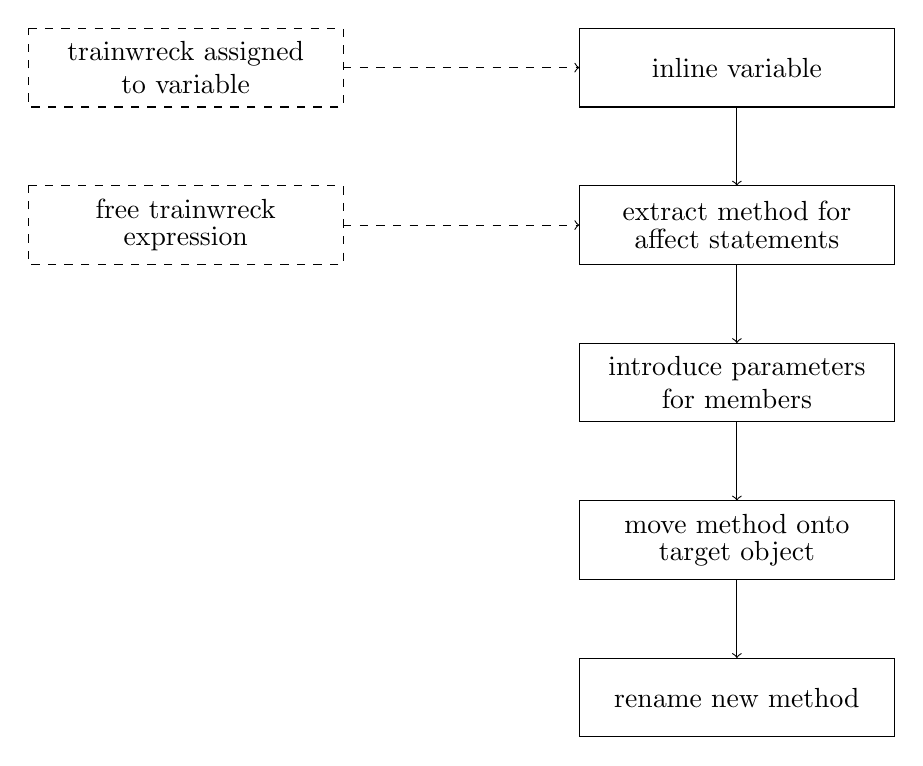
\begin{tikzpicture}
                        \draw
                        (4, -0.5) edge[->, dashed] (7, -0.5)
                        (4, -2.5) edge[->, dashed] (7, -2.5)
                        (9, -1) edge[->] (9, -2)
                        (9, -3) edge[->] (9, -4)
                        (9, -5) edge[->] (9, -6)
                        (9, -7) edge[->] (9, -8);
                        \begin{scope}[shift={(0, 0)}]
                            \node at (2, -0.5) {\shortstack{trainwreck assigned\\to variable}};
                            \draw[dashed] (0, 0) -- (4, 0) -- (4, -1) -- (0, -1) -- cycle;
                        \end{scope}
                        \begin{scope}[shift={(0, -2)}]
                            \node at (2, -0.5) {\shortstack{free trainwreck\\expression}};
                            \draw[dashed] (0, 0) -- (4, 0) -- (4, -1) -- (0, -1) -- cycle;
                        \end{scope}
                        \begin{scope}[shift={(7, 0)}]
                            \node at (2, -0.5) {inline variable};
                            \draw (0, 0) -- (4, 0) -- (4, -1) -- (0, -1) -- cycle;
                        \end{scope}
                        \begin{scope}[shift={(7, -2)}]
                            \node at (2, -0.5) {\shortstack{extract method for\\affect statements}};
                            \draw (0, 0) -- (4, 0) -- (4, -1) -- (0, -1) -- cycle;
                        \end{scope}
                        \begin{scope}[shift={(7, -4)}]
                            \node at (2, -0.5) {\shortstack{introduce parameters\\for members}};
                            \draw (0, 0) -- (4, 0) -- (4, -1) -- (0, -1) -- cycle;
                        \end{scope}
                        \begin{scope}[shift={(7, -6)}]
                            \node at (2, -0.5) {\shortstack{move method onto\\target object}};
                            \draw (0, 0) -- (4, 0) -- (4, -1) -- (0, -1) -- cycle;
                        \end{scope}
                        \begin{scope}[shift={(7, -8)}]
                            \node at (2, -0.5) {rename new method};
                            \draw (0, 0) -- (4, 0) -- (4, -1) -- (0, -1) -- cycle;
                        \end{scope}
                    \end{tikzpicture}
                \end{center}
            \subsubsection*{Defending against Null Pointer Exceptions}
                The following snippet of code has lines 3 and 5 added to protect against NPEs - however if this is needed frequently it could lead to code duplication;
                \begin{lstlisting}
                    void playTrack(String name) {
                      Track track = library.getTrack(name);
                      if (track != null) {
                        track.play();
                      }
                    }
                \end{lstlisting}
                Another approach is to have the \textbf{null object pattern}, which is an empty implementation;
                \begin{lstlisting}
                    interface Track {
                      public void play();
                    }

                    class NullTrack implements Track {
                      public void play() {
                        // do nothing
                      }
                    }
                \end{lstlisting}
                As a development team, it makes sense to agree on what will be done, whether it be using the null object pattern, or using Java's ~Optional~s.
            \subsubsection*{Coupling and Cohesion}
                \begin{itemize}
                    \itemsep0em
                    \item aim for \textbf{low coupling} between classes \hfill changing one part requires a change in the other
                    \item aim for \textbf{high cohesion} within each class \hfill a class should be specialised (less changes needed)
                \end{itemize}
                Ideally, we want to limit the "blast radius" of our changes, which is the amount of code we affect to just parts managed by us.
            \subsubsection*{Approaches}
                One extreme is to store all of the code in a single repository, allowing changes to be made when needed (given approval), which is done by Google.
                This has the benefit that a part can be changed in part of the code, and can also be fixed in another.
                However, due to the ability to affect other unrelated parts of the codebase, it can also lead to issues when updating a core object.
                \medskip

                The other extreme is to have modular code, which is individually versioned.
                That way, if something is updated, other modules can use older versions and update when needed (which doesn't break functionality straight away).
                However, updates will need to be done quite frequently, otherwise other modules will be behind.
                It's also difficult to make changes in other parts.
        \subsection*{22nd October 2019}
            \subsubsection*{Motivation}
                This focuses mostly on the middle two layers in the pyramid mentioned in the first lecture.
                We assume that the code is working correctly, and we can check that the code is working correctly with the test suite.
            \subsubsection*{Example}
                ~ReverseEncoder~ is an encoder for encryption, which reverses each word in the input (such that ~"abc 123"~ becomes ~"cba 321"~).
                This will be done in Python;
                \begin{lstlisting}
                    class ReverseEncoder:
                      def encode(self, line):
                        words = line.split(" ")
                        results = []
                        for word in words:
                          results.append(word[::-1])
                        return " ".join(results)
                \end{lstlisting}
                Now suppose we have another encoder, ~DoublingEncoder~, that repeats each word in the input (such that ~"abc 123"~ becomes ~"abcabc 123123"~).
                This can easily be implemented as follows;
                \begin{lstlisting}
                    class DoublingEncoder:
                      def encode(self, line):
                        words = line.split(" ")
                        results = []
                        for word in words:
                          results.append(word + word)
                        return " ".join(results)
                \end{lstlisting}
                However, notice that there is a significant amount of duplication, as essentially all lines are the same, other than line 6.
                To remedy this, we can add an ~Encoder~ class which they both extend;
                \begin{lstlisting}
                    from abc import abstractmethod

                    class Encoder:
                      def encode(self, line):
                        words = line.split(" ")
                        results = []
                        for word in words:
                          results.append(self.encode_word(word))
                        return " ".join(results)

                      @abstractmethod
                      def encode_word(self, word):
                        pass

                    class ReverseEncoder(Encoder):
                      def encode_word(self, word):
                        return word[::-1]

                    class DoublingEncoder(Encoder):
                      def encode_word(self, word):
                        return word + word
                \end{lstlisting}
                Now, everything that is common to the two algorithms is in the superclass, and only the part that is specialised is each individual class.
            \subsubsection*{Template Method Pattern}
                The template method pattern is used when requirements change over time, and we need to vary a small part of an algorithm.
                A skeleton should be defined (our ~Encoder~ in the example above), and the vary steps should be deferred to subclasses (~ReverseEncoder~, and ~DoublingEncoder~).
                \begin{center}
                    Separate things that change from things that stay the same.
                \end{center}
                Generally, this has the following pattern, where the specialised \teal{hook methods} are overwritten by the \blue{inheriting} classes, and the \violet{template method} contains the shared behaviour;
                \begin{center}
                    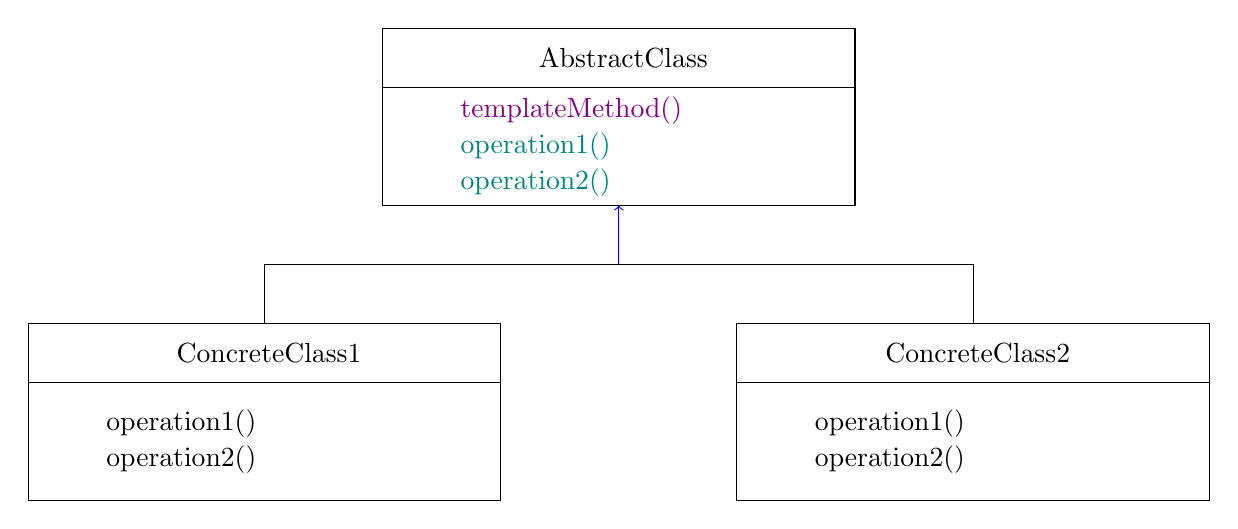
\begin{tikzpicture}[x=1.5cm, y=0.75cm]
                        \begin{scope}[shift={(0, 0)}]
                            \node at (2, -0.5) {~AbstractClass~};
                            \node[anchor=west] at (0.5, -2) {\shortstack[l]{\violet{~templateMethod()~}\\\teal{~operation1()~}\\\teal{~operation2()~}}};
                            \draw
                            (0, 0) -- (4, 0) -- (4, -3) -- (0, -3) -- cycle
                            (0, -1) -- (4, -1);
                        \end{scope}
                        \begin{scope}[shift={(-3, -5)}]
                            \node at (2, -0.5) {~ConcreteClass1~};
                            \node[anchor=west] at (0.5, -2) {\shortstack[l]{~operation1()~\\~operation2()~}};
                            \draw
                            (0, 0) -- (4, 0) -- (4, -3) -- (0, -3) -- cycle
                            (0, -1) -- (4, -1);
                        \end{scope}
                        \begin{scope}[shift={(3, -5)}]
                            \node at (2, -0.5) {~ConcreteClass2~};
                            \node[anchor=west] at (0.5, -2) {\shortstack[l]{~operation1()~\\~operation2()~}};
                            \draw
                            (0, 0) -- (4, 0) -- (4, -3) -- (0, -3) -- cycle
                            (0, -1) -- (4, -1);
                        \end{scope}
                        \draw
                        (-1, -5) -- (-1, -4) -- (5, -4) -- (5, -5)
                        (2, -4) edge[->, blue] (2, -3);
                    \end{tikzpicture}
                \end{center}
                This follows the \textbf{open-closed principle}, where we can extend the class' behaviour without modifying it, as we can just add a new subclass.
                We therefore don't have to edit code, which may have lead to bugs, as we are safer by just adding code.
                Modules should be open for extension, but closed to modification.
                Change behaviour by adding new code, not by changing existing code.
            \subsubsection*{Coupling Metrics}
                Afferent coupling (Ca) - remember this as how many arrows \textbf{a}rrive - a class' afferent couplings is a measure of it's responsibility (how many other classes use it).
                Efferent coupling (Ce) - remember this as how many arrows \textbf{e}xit - it's a measure of how many different classes are used by this specific class (measures independence).
                \medskip

                For example, the ~ReverseEncoder~ cannot really be used elsewhere, as it has a strong coupling with the ~Encoder~ superclass.
                In general, we may want to avoid this coupling.
            \subsubsection*{Strategy Pattern}
                An alternative is the template method (still done for the same reason) is to delegate to a collaborator (instead of a subclass) - the algorithm should be pulled into a separate object.
                This favours object composition over class inheritance.
                \begin{center}
                    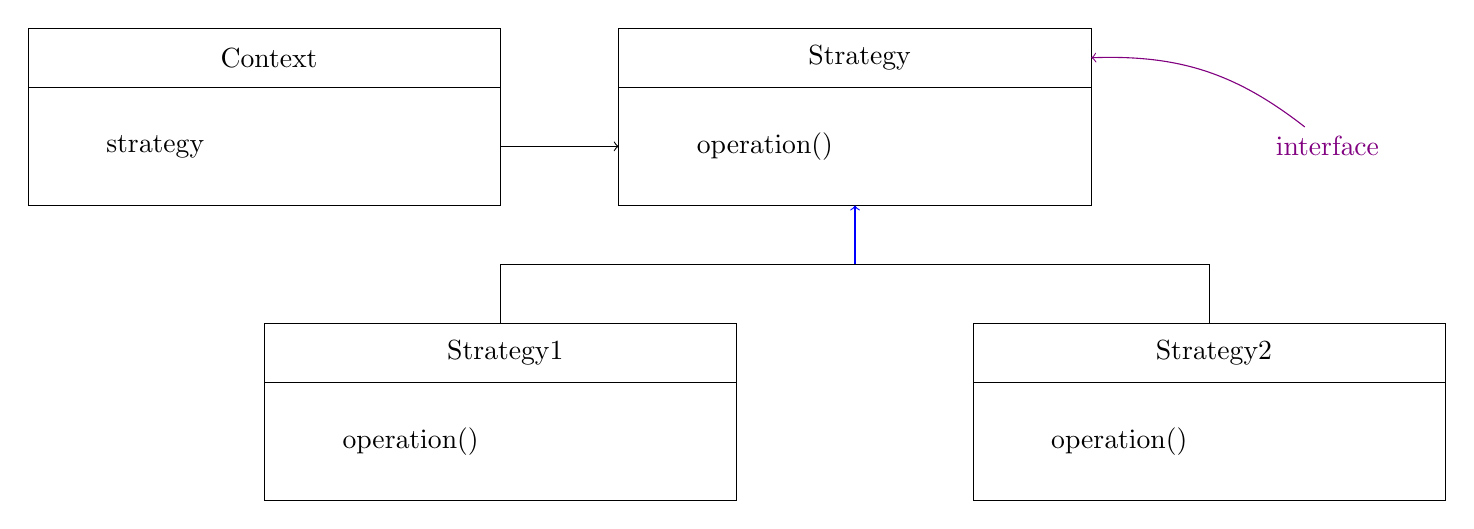
\begin{tikzpicture}[x=1.5cm, y=0.75cm]
                        \begin{scope}[shift={(-5, 0)}]
                            \node at (2, -0.5) {~Context~};
                            \node[anchor=west] at (0.5, -2) {~strategy~};
                            \draw
                            (0, 0) -- (4, 0) -- (4, -3) -- (0, -3) -- cycle
                            (0, -1) -- (4, -1);
                        \end{scope}
                        \begin{scope}[shift={(0, 0)}]
                            \node at (2, -0.5) {~Strategy~};
                            \node[anchor=west] at (0.5, -2) {~operation()~};
                            \draw
                            (0, 0) -- (4, 0) -- (4, -3) -- (0, -3) -- cycle
                            (0, -1) -- (4, -1);
                        \end{scope}
                        \begin{scope}[shift={(-3, -5)}]
                            \node at (2, -0.5) {~Strategy1~};
                            \node[anchor=west] at (0.5, -2) {~operation()~};
                            \draw
                            (0, 0) -- (4, 0) -- (4, -3) -- (0, -3) -- cycle
                            (0, -1) -- (4, -1);
                        \end{scope}
                        \begin{scope}[shift={(3, -5)}]
                            \node at (2, -0.5) {~Strategy2~};
                            \node[anchor=west] at (0.5, -2) {~operation()~};
                            \draw
                            (0, 0) -- (4, 0) -- (4, -3) -- (0, -3) -- cycle
                            (0, -1) -- (4, -1);
                        \end{scope}
                        \node[violet] at (6, -2) (i) {interface};
                        \draw
                        (i) edge[->, violet, bend right=20] (4, -0.5)
                        (-1, -2) edge[->] (0, -2)
                        (-1, -5) -- (-1, -4) -- (5, -4) -- (5, -5)
                        (2, -4) edge[->, blue] (2, -3);
                    \end{tikzpicture}
                \end{center}
                It's important to note that ~Strategy~ is an interface, hence ~Strategy1~ and ~Strategy2~ implement it.
                The example can be modified as follows;
                \begin{lstlisting}
                    from abc import abstractmethod

                    class Encoder:
                      def __init__(self, encryptor):
                        self.encryptor = encryptor

                      def encode(self, line):
                        words = line.split(" ")
                        results = []
                        for word in words:
                          results.append(self.encryptor.encode_word(word))
                        return " ".join(results)

                    class Reverser:
                      def encode_word(self, word):
                        return word[::-1]

                    class Doubler:
                      def encode_word(self, word):
                        return word + word
                \end{lstlisting}
                The main sign is that the strategy is passed in to the context; hence we would have;
                \begin{center}
                    ~Encoder(Reverser()).encode("...")~
                \end{center}
                As the ~Reverser~ and ~Doubler~ no longer have a relationship with ~Encoder~, we have must less coupling, hence we have better mobility and flexibility.
                Generally, composition should be preferred over inheritance.
        \subsection*{25th October 2019}
            \subsubsection*{Stability}
                If a core object, such as a ~Customer~ class, has many things depending on it, such that it has a high afferent coupling, it can be a benefit since it can be heavily reused.
                However, it needs to be very stable, and require little to no changing, as changing it can break other parts of the codebase if done incorrectly.
                It should rely on very few other objects (if any).
                These are represented by the \teal{\textbf{teal}} nodes below.
                \medskip

                On other hand, the components at the edges (the ones in \textbf{\violet{violet}}), can include UI components, such as a dashboard.
                It makes sense for the dashboard to depend on the ~Customer~ class, but not the other way around.
                These can be changed fairly easily, as not many things depend on it.
                \begin{center}
                    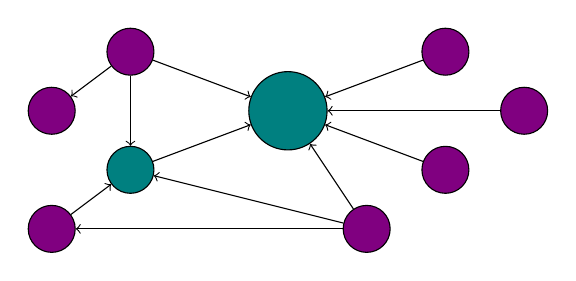
\begin{tikzpicture}[y=0.75cm]
                        \node[inner sep=10pt, circle, draw=black, fill=teal] (t1) at (0, 0) {};
                        \node[inner sep=6pt, circle, draw=black, fill=teal] (t2) at (-2, -1) {};
                        \node[inner sep=6pt, circle, draw=black, fill=violet] (p1) at (-3, 0) {};
                        \node[inner sep=6pt, circle, draw=black, fill=violet] (p2) at (-2, 1) {};
                        \node[inner sep=6pt, circle, draw=black, fill=violet] (p3) at (-3, -2) {};
                        \node[inner sep=6pt, circle, draw=black, fill=violet] (p4) at (1, -2) {};
                        \node[inner sep=6pt, circle, draw=black, fill=violet] (p5) at (3, 0) {};
                        \node[inner sep=6pt, circle, draw=black, fill=violet] (p6) at (2, 1) {};
                        \node[inner sep=6pt, circle, draw=black, fill=violet] (p7) at (2, -1) {};
                        \draw
                        (t2) edge[->] (t1)
                        (p2) edge[->] (t1) (p2) edge[->] (t2) (p2) edge[->] (p1)
                        (p3) edge[->] (t2)
                        (p4) edge[->] (t1) (p4) edge[->] (t2) (p4) edge[->] (p3)
                        (p5) edge[->] (t1)
                        (p6) edge[->] (t1)
                        (p7) edge[->] (t1);
                    \end{tikzpicture}
                \end{center}
            \subsubsection*{Complexity Metrics}
                Some methods for quantifying the complexity of a program are as follows;
                \begin{itemize}
                    \itemsep0em
                    \item \textbf{cyclomatric (McCabe)}
                        \medskip

                        Described in McCabe's paper, it counts the possible different executions that could happen, and gives a lower bound on the number of tests required for a particular unit.
                    \item \textbf{WILT (Whitespace Integrated over Lines of Text)}
                        \medskip

                        Integrates over the indented area of a given piece of code - this has a correlation with the McCabe complexity, but is much easier to calculate.
                    \item \textbf{ABC (Assignments, Branches, and Conditions)}
                        \medskip

                        Every time it encounters each of the following constructs, it increments a counter by some number.
                        This isn't as accurate as McCabe, but gives an approximation.
                        For example, \textit{Flog} is an ABC metric with specialist knowledge of Ruby;
                        \begin{lstlisting}
                            def blah         # 11.2 total
                              a = eval "1+1" # 1.2 (a=) + 6.0 (eval) +

                              if a == 2      # 1.2 (if) + 1.2 (==) + 0.4 (fixnum) +
                                puts "yay"   # 1.2 (puts)
                              end
                            end
                        \end{lstlisting}
                \end{itemize}
                I honestly have no idea what this lecture is supposed to be going through.
                Generally, we should look at the trends for the complexity of code, rather than ensuring it is monotonically improving.
            \subsubsection*{Turbulence}
                If we plot complexity against commits (number of changes), we can divide it into 4 general quadrants.
                Something that is high complexity, but has low commits, probably doesn't need to be refactored as we aren't modifying it often.
                This could be an algorithm copied from an academic paper, or a third party library being imported.
                The quadrant with low complexity and high commits could include configuration files, which are modified frequently.
                \medskip

                The top right quadrant, which has high complexity and high commits should be a cause for concern.
                This is likely to introduce bugs as it is being changed often, and has high complexity.
        \subsection*{29th October 2019}
            \subsubsection*{Factory Method Pattern}
                Factory methods (along with objects) allow for more flexibility and clarity with regards to object creation.
                Factory methods can have names unlike constructors.
                Note that the example on line 5 should be motivation to use factory methods, as it has less clarity, compared to the line above.
                By doing this, we can also close off some options by not exposing the constructor.
                \begin{lstlisting}
                    List<Object> l = Collections.emptyList();
                    Boolean b = Boolean.valueOf("true");
                    ExecutorService es = Executors.newFixedThreadPool(4);
                    VirtualMachine vm1 = VirtualMachine.withHardDiskGigabytes(128);
                    // VirtualMachine vm2 = new VirtualMachine(2, 512, 128);
                \end{lstlisting}
                The ~VirtualMachine~ example can be done as follows;
                \begin{lstlisting}
                    class VirtualMachine {

                      private final int cores;
                      private final int ram;
                      private final int disk;
                      private final int costPerMin;
                      ...

                      // factory methods are static
                      public static VirtualMachine withHardDiskGigabytes(int size) {
                        return new VirtualMachine(4, 128, size);
                      }

                      // private constructors force callers to use the factory methods
                      private VirtualMachine(int cores, int ram, int disk) {
                        this.cores = cores;
                        this.ram = ram;
                        this.disk = disk;
                        this.costPerMin = (cores * ram + disk) / 50;
                        ...
                      }
                    }
                \end{lstlisting}
            \subsubsection*{Factory Objects}
                Sometimes, we don't know what we want to display until run-time (and therefore can't put it in directly) - as such, factory objects can decide what to return at run-time (example for some UI);
                \begin{lstlisting}
                    class LogoFactory {

                      // can return any sub-type of Logo
                      static Logo createLogo() {
                        if (config.country().equals(Country.UK)) {
                          return new FlagLogo("UK");
                        }
                        if (config.country().equals(Country.USA)) {
                          return new FlagLogo("US");
                        }
                        return new DefaultLogo();
                      }

                      class FlagLogo implements Logo { ... }
                      class DefaultLogo implements Logo { ... }
                    }
                \end{lstlisting}
                Therefore, when we need the logo, we can call ~LogoFactory.createLogo()~ to obtain the appropriate one.
                Additionally, if we want to add a new logo, it only needs to be modified in one place.
            \subsubsection*{Abstract Factory Pattern}
                This is less frequently used.
                It's an interface of a factory, thus all implementations of it are factories.
                \begin{lstlisting}
                    interface WidgetFactory {
                      Widget createScrollBar();
                      Widget createMenu();
                      ...
                    }

                    class MobileWidgetFactory implements WidgetFactory {

                      @Override
                      public Widget createScrollBar() {
                        return new MobileScrollBar(Color.GREEN);
                      }

                      @Override
                      public Widget createMenu() {
                        return new MobileMenu(5);
                      }
                      ...
                    }

                    class DesktopWidgetFactory implements WidgetFactory {

                      @Override
                      public Widget createScrollBar() {
                        ...
                      }
                      ...
                    }
                \end{lstlisting}
                This can help maintain consistency (such that we don't get a ~MobileScrollBar~ when building a desktop UI, etc).
            \subsubsection*{Builder Pattern}
                Separate the construction of a complex object, likely with many parameters, from its representation.
                We also want the object to be in a "usable state" once it is first constructed, such that we don't have a transitionary state.
                An example is as follows;
                \begin{lstlisting}
                    public class BananaBuilder {

                      private double ripeness = 0.0;
                      private double curve = 0.5;

                      // ensures the builder itself is created with factory method
                      private BananaBuilder() { }

                      public static BananaBuilder aBanana() {
                        return new BananaBuilder();
                      }

                      public Banana build() {
                        Banana banana = new Banana(curve);
                        banana.ripen(ripeness);
                        return banana;
                      }

                      public BananaBuilder withRipeness(double ripeness) {
                        this.ripeness = ripeness;
                        return this;
                      }

                      public BananaBuilder withCurve(double curve) {
                        this.curve = curve;
                        return this;
                      }
                    }
                \end{lstlisting}
                Note that the configuration methods return ~this~ (and is mutable), which gives a fluent interface allowing for method chaining.
                The builder can be used as follows;
                \begin{lstlisting}
                    import static BananaBuilder.*

                    public class FruitBasket {
                      ...

                      public FruitBasket() {
                        Banana banana = aBanana().withRipeness(2.0).withCurve(0.9).build();
                        ...
                      }
                    }
                \end{lstlisting}
                The ~build()~ method also allows us to validate the parameters (which can also have default values).
            \subsubsection*{Singleton Pattern}
                We often do not need this pattern, and it can be troublesome when misused.
                The singleton pattern ensures a class only has one instance, and there is a global point of access - this is typically when instantiating the object has a high cost (high memory cost, actual fee, etc).
                An example of this is as follows;
                \begin{lstlisting}
                    public class BankAccountStore {

                      // static initialisation runs when class loaded
                      private static BankAccountStore instance = new BankAccountStore();

                      private Collection<BankAccount> accounts;

                      // private constructor ensures no-one can create a new instance
                      private BankAccountStore() {
                        ...
                      }

                      // getInstance() is called to gain access to the global instance
                      public static BankAccountStore getInstance() {
                        return instance;
                      }

                      public BankAccount lookupAccountById(int id) {
                        ...
                      }
                      ...
                    }
                \end{lstlisting}
                The example above is an eager initialisation, which could be wasteful if it has a high cost to initialise, but no one actually needs it;
                \begin{lstlisting}
                    public class BankAccountStore {

                      // no initialisation when class loaded
                      private static BankAccountStore instance;

                      private Collection<BankAccount> accounts;

                      // private constructor ensures no-one can create a new instance (expensive)
                      private BankAccountStore() {
                          ...
                      }

                      // getInstance() is called to gain access to the global instance
                      public static synchronized BankAccountStore getInstance() {
                        if (instance == null) {
                          instance = new BankAccountStore();
                        }
                        return instance;
                      }

                      public BankAccount lookupAccountById(int id) {
                        ...
                      }
                      ...
                    }
                \end{lstlisting}
                Note that we have made the method thread-safe to avoid the race condition where multiple threads attempt to create instances simultaneously.
            \subsubsection*{Dependencies}
                Note that in the example below, we have a strong coupling between a ~PushSwitch~ and a ~Light~.
                This means that we cannot really test the switch independently of the light - which we want to avoid.
                Additionally, we cannot use this switch for another device, if required.
                \begin{lstlisting}
                    class Light:
                      def on(self):
                        print("Shining")

                      def off(self):
                        print("Dark")

                    class PushSwitch:
                      def __init__(self):
                        self.light = Light();
                        self.on = False

                      def press(self):
                        self.on = not self.on
                        if self.on:
                          self.light.on()
                        else
                          self.light.off()

                    switch = PushSwitch()
                \end{lstlisting}
                The fix for this is following the \textbf{dependency-inversion principle} - we want to depend upwards on an abstraction, rather than downwards on a concrete class.
                \begin{lstlisting}
                    class PushSwitch:
                      def __init__(self, device):
                        self.device = device
                        self.on = False

                      def press(self):
                        self.on = not self.on
                        if self.on:
                          self.device.on()
                        else
                          self.device.off()

                      switch = PushSwitch(Light())
                \end{lstlisting}
                However, singleton creates dependency, and if we wanted to run unit tests, we would need the actual singleton instance in production (which may be sensitive, and cannot be tested on).
                It doesn't allow us to create mock objects.
\end{document}
